\documentclass[crop,tikz]{standalone}

\usepackage{tikz}
\usepackage{anyfontsize}

\usetikzlibrary{bending}
\usetikzlibrary{arrows.meta}
\begin{document}

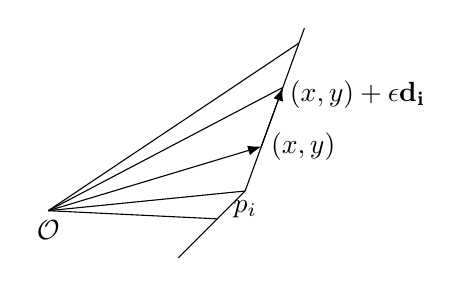
\begin{tikzpicture}

\draw ([shift=(-135:1.2)]1.5,0.5) -- (1.5,0.5);
\node [below] at (1.5,0.5) {$p_i$};
\draw (1.5,0.5) -- ([shift=(70:2.2)]1.5,0.5);

\draw [-Latex] (-1,0.25) -- ([shift=(70:0.6)]1.5,0.5);

\draw (-1,0.25) -- (1.5,0.5);
\draw (-1,0.25) -- ([shift=(-135:0.5)]1.5,0.5);
\draw (-1,0.25) -- ([shift=(70:1.4)]1.5,0.5);
\draw (-1,0.25) -- ([shift=(70:2)]1.5,0.5);

\draw [-Latex] ([shift=(70:0.6)]1.5,0.5) -- ([shift=(70:1.4)]1.5,0.5);

\node [below] at (-1, 0.25) {$\mathcal{O}$};
\node [right] at ([shift=(70:0.6)]1.5,0.5) {$(x, y)$};
\node [right] at ([shift=(70:1.3)]1.5,0.5) {$(x,y) + \epsilon \bf{d}_i$};


\end{tikzpicture}

\end{document}